\section{Heat and momentum sources}\label{heat-and-momentum-sources}

Consider for the moment a seminfinite atmoshere over a flat surface. The
flow is determined by the conservation of quasi-geostrophic potential
vorticity that we can write in terms of a conservation law as

\[\frac{\partial q}{\partial t} = -\nabla\cdot(\mathbf{v}_g q)\]

the equation needs a boundary condition for the solution that is
provided by the temperature equation, eq. (\texttt{qgTempBC})

\[\frac{\partial }{\partial t}\frac{\partial \psi}{\partial z} = -J(\psi, \frac{\partial \psi}{\partial z}) \qquad  at  \qquad z=0\]

Operating with \(\frac{\partial }{\partial y}\) on eq. \texttt{eq:qg} we
obtain an equation for the tendency of the zonal wind

\[\chi = \frac{\partial u}{\partial t} \qquad u =-\frac{\partial \psi}{\partial y}\]

\[\nabla^2 \chi + f_0\frac{\partial }{\partial z}\frac{1}{N^2}\frac{\partial \chi}{\partial z} = -\frac{\partial }{\partial y} \nabla\cdot(\mathbf{v}_g q)\]

in the same way we can differentiate the boundary condition

\[\frac{\partial \chi}{\partial z}= -\frac{1}{f_0}\frac{\partial }{\partial y} \nabla\cdot(\mathbf{v}_g \theta) \qquad  at  \qquad z=0\]

together these two equation are an elliptic system that can be solved.
The boundary condition is somewhat complicated. A standard method is to
include the condition in the interior of the fluid by adding a term with
a \(\delta\) function that allows to have a Dirichlet boundary condition
for the elliptic problem, i.e. \(\frac{\partial \chi}{\partial z} = 0\)
at \(z=0\). The interior equation then becomes

\[\nabla^2 \chi + f_0\frac{\partial }{\partial z}\frac{1}{N^2}\frac{\partial \chi}{\partial z} = -\frac{\partial }{\partial y} \nabla\cdot\left( \mathbf{v}_g q +\frac{f_0}{N^2} \mathbf{v}_g\theta \delta(z^+) \right)\]

A similar process will yield the equation for the temperature tendency,
by using this this the z-derivative of eq. (\texttt{eq:qg})

\[\phi = \frac{\partial \theta}{\partial t} =f_0\frac{\partial }{\partial t}\frac{\partial \psi}{\partial z}\]

or

\[
\nabla^2\phi + f_0^2 \frac{\partial^{2}}{\partial z^{2}} \frac{1}{N^2} \phi = f_0\frac{\partial }{\partial z}\nabla\cdot(\mathbf{v}_g \theta)
\]

Taking the zonal mean of eq. (\texttt{eq:chi}) and (\texttt{eq:phi}) we
obtain

\[\begin{aligned}
\frac{\partial^{2} \bar{\chi}}{\partial y^{2}} + f_0^2 \frac{\partial }{\partial z} \frac{1}{N^2} \frac{\partial \bar{\chi}}{\partial z} &=\frac{\partial^{2} }{\partial y^2} \left( \overline{v_g q} + \frac{f_0}{N^2} \overline{v_g\theta} \delta(z^+) \right)  \\
\frac{\partial^{2} \bar{\phi}}{\partial y^{2}} +f_0^2 \frac{\partial }{\partial z} \frac{1}{N^2} \frac{\partial \bar{\phi}}{\partial z} &= -f_0 \frac{\partial^{2} }{\partial {y}\partial{z}} \overline{v_g q}
\end{aligned}\]

with the boundary condition

\[\bar{\phi}= -\frac{\partial }{\partial y}\overline{v_g\theta} \qquad  at z=0.\]

We can understand how these equation works by going back to the QG
equation of motion (\texttt{eq:eqmotion}) and apply a zonal average

\[\begin{aligned}
\frac{\partial \bar{u}}{\partial t} &= f_0 \bar{v}-\frac{\partial }{\partial y}\overline{u'v'} + \cal{F} \\
\frac{\partial \bar{\theta}}{\partial t} &= -N^2 \bar{w}-\frac{\partial }{\partial y}\overline{v'\theta'} + \cal{H} \\
f_0\frac{\partial \bar{u}}{\partial z} &= -\frac{\partial \bar{\theta}}{\partial y}\\
\frac{\partial \bar{v}}{\partial y} &= -\frac{\partial \bar{w}}{\partial z}
\end{aligned}\]

where we have added a momentum forcing \(\cal{F}\) and and a heating
forcing \(\cal{H}\). (Check the residual circulation issue). We can
include the nonlinear fluxes into the forcings, redefining the forcings
as

\[
\begin{aligned}
\widetilde{\mathcal{F}} &= \mathcal{F} -\frac{\partial}{\partial y} \overline{u'v'} \\
\widetilde{\mathcal{H}} &= \mathcal{H} -\frac{\partial }{\partial y} \overline{u'\theta'}
\end{aligned}
\]

the last two equations can be used to eliminate the vertical and
meridional velocities to obtain a close system for the meridional
circulation in terms of \(\bar{u}\) and \(\bar{\theta}\). Cross
derivating Eq.(\texttt{eq:uvtheta}) we obtain the equation

\[
f_0^2 \frac{\partial^{2} \Phi}{\partial z^{2}} + N^2 \frac{\partial^{2} \Phi}{\partial y^2} =
-f_0\frac{\partial \mathcal{F}}{\partial z} - \frac{\partial \mathcal{H}}{\partial y}
\]
that implies a streamfunction for the meridional circulation

\[(\bar{v},\bar{w}) = \left( \frac{\partial \Phi}{\partial z},-\frac{\partial \Phi}{\partial y}\right)\]

This equation can be solved for \(\bar{v},\bar{w}\) (with suitable
boundary conditions, for instance \(\Phi = 0\) at the lower flat
boundary) and then used to compute the zonal and temperature changes of
the basic state from eq. \texttt{eq:uvmean}. We can then see that
meridional fluxes are essential to maintain the geostrophic balance of
the basic state and they are equivalent to a meridional circulation. It
is interesting to note that the circulation is determined by an elliptic
(\texttt{eq:elliptic}) that is one of the reason for the nonlocal
character fo the response to forcings.

\subsection{The meridional response to
forcings}\label{the-meridional-response-to-forcings}

The meridional circulation equation is a two-dimensional Poisson
equation that can be solved using the Green's function method. The
Green's function is

\[G(\mathbf{r},\mathbf{r}_0) = \frac{1}{2\pi} \log(| \mathbf{r}-\mathbf{r}_0|)\]

the equation can be simplified somewhat re-defining \(z\) as
\(\frac{ N z}{f_0}\). considering \(N^2\) constant,

\[
\frac{\partial^{2} \Phi}{\partial z^{2}} + \frac{\partial^{2} \Phi}{\partial y^2} =
-\frac{f_0}{N^2}\frac{\partial \mathcal{F}}{\partial z} - \frac{1}{N^2}\frac{\partial \mathcal{H}}{\partial y}
\]

so the solution to the forced problem can be written as
\[
\Phi(y,z) = \frac{1}{2\pi}\int dy_0 dz_0 \log( R) 
\left[ -\frac{f_0}{N^2}\frac{\partial \mathcal{F}}{\partial z} - \frac{1}{N^2}\frac{\partial \mathcal{H}}{\partial y} \right]
\]

where \(R^2 = (y-y_0)^2 + (z-z_0)^2\) Consider first the case of only
heating \(\mathcal{F} = 0\), then

\[
\Phi(y,z) = -\frac{1}{2\pi N^2}\int dy_0 dz_0 \log( R)  \frac{\partial \mathcal{H}}{\partial y}(y_0,z_0)
\]

integrating by parts and using the boundary condition

\[\Phi(y,z) = \frac{1}{2\pi N^2}\int dy_0 dz_0 \frac{\partial }{\partial y}\log( R) \mathcal{H}(y_0,z_0)\]

or

\[\Phi(y,z) = \frac{1}{2\pi N^2}\int dy_0 dz_0 \frac{(y_0-y) }{R^2} \mathcal{H}(y_0,z_0)\]

assuming a delta function source \( \mathcal{H} = A \delta (0)\) we obtain
the solution for the meridional streamfunction response to a localized
heating

\[\Phi(y,z) = -\frac{A}{2\pi N^2} \frac{y}{R^2}\]

with a corresponding circulation

\[\begin{aligned}
w &= -\frac{\partial \Phi}{\partial y} =\frac{A}{2\pi N^2} \frac{1}{R^2}\left( 1 -2(\frac{y}{R})^2 \right) \\
v &= \frac{f_0}{N^2}\frac{\partial \Phi}{\partial z} =\frac{Af_0}{\pi N^3} \frac{y z}{R^4}
\end{aligned}\]

\begin{figure}
\centering
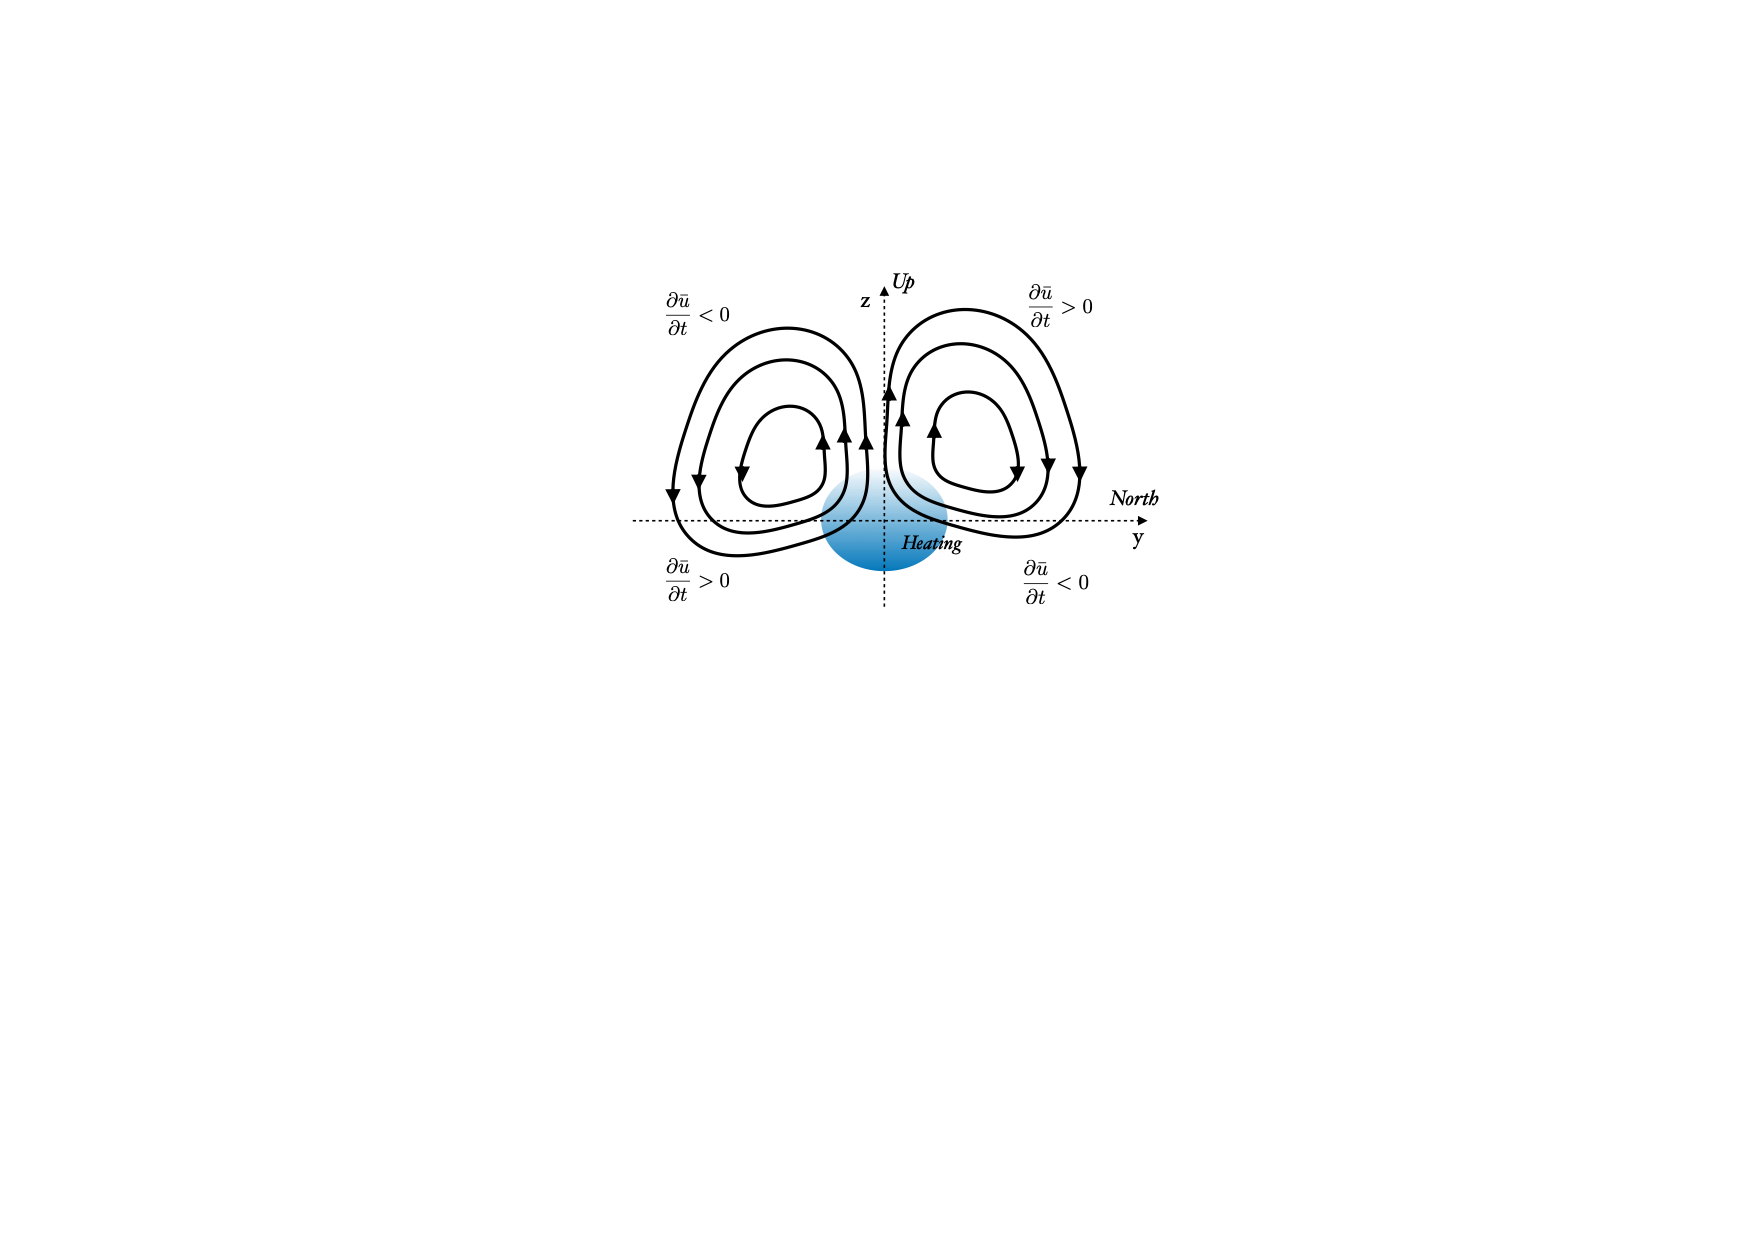
\includegraphics[width = .7 \textwidth]{figs/GD/Hforcing.png}
\caption{}
\end{figure}

The circulation response in the meridional plane consist of raising
motion in the location of the heating, with compensating branches north
and south. The flow converges at low levels at the heating location and
divergence is generated aloft.

A similar analysis can be done for the case of momentum forcing, if
assume a positive localized momentum frorcing as before, simple symmetry
calculation lead to the response in Fig. (\texttt{fig:62})

\begin{figure}
\centering
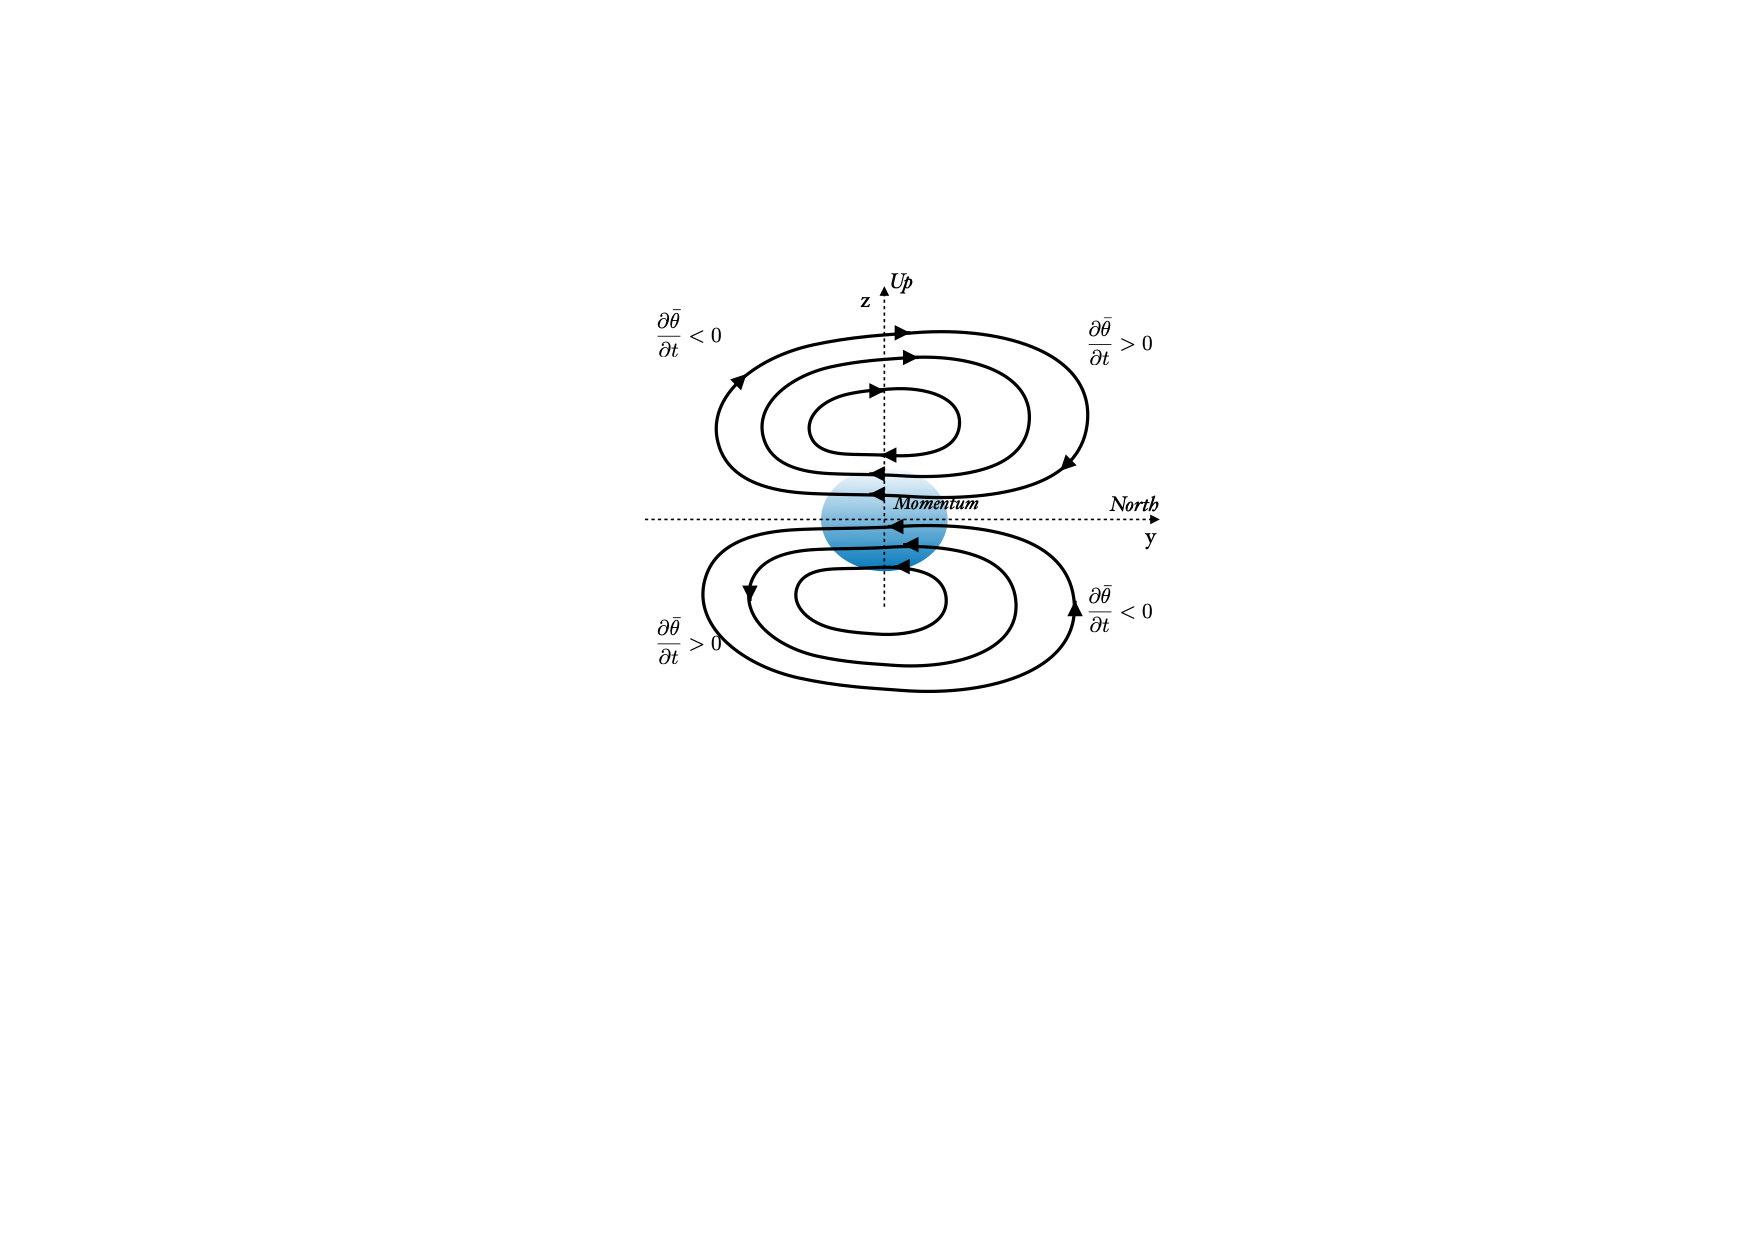
\includegraphics[width = .7 \textwidth]{figs/GD/FForcing.png}
\caption{}
\label{fig:}
\end{figure}

In this case the meridional circulation in response to a positive
(westerly) momentum source is aequatorward motion that creates a
meridional cell circulation south of the source of momentum. The
meridional flow partially compensate for the westerly momentum input at
higher latitudes. The teperature changes accordingly to maintain thermal
wind balance.

However, is is important to note that in both cases, because of the
geostrophic and thermal wind balance, both a wind and a temperature
response will be generated. it is therefore interesting to try to
understand what is the relative separation between these two responses.
We can use the system of equation (\texttt{eq:uvmean}) to write an
equation for the temperature tendency

\[\phi = \frac{\partial \bar{\theta}}{\partial t}\]

obtaining
\[
\frac{\partial^{2} \phi}{\partial y^{2}} + f_0^2\frac{\partial^{2} }{\partial z^{2}} \frac{\phi}{N^2} = 
-f_0 \frac{\partial }{\partial z} \left( \frac{\partial \widetilde{\mathcal{F}}}{\partial y} -f_0 \frac{\partial }{\partial z} \frac{\widetilde{\mathcal{H}}}{N^2} \right)
\]

suppose that \( \widetilde{\mathcal{F}} \approx 0\) and
\(\widetilde{\mathcal{H}} = \widetilde{\mathcal{H}}_0 \sin{m z}\) then
\(\phi \approx \phi_0 \sin{m z}\) and

\[
\frac{L}{\lambda_m^2} \frac{\partial^{2} \phi}{\partial y^{2}} - \phi_0 =  \widetilde{\mathcal{H}}_0
\]

where \(\lambda_m^2 = \frac{N}{f_0 m}\) is a scale linked to the
stratification and the verticalscale of the forcing, in this context is
the relevant deformation radius. The eq. (\texttt{eq:deform}) provides a
scale ratio. In a linear sense the horizontal scale of the forcing
\(\widetilde{\mathcal{H}}\) fixes the horizontal scale \(L\) of the
response, so if this scale is much larger than the deformation the
dominant balance is

\[\phi_0 \approx  \widetilde{\mathcal{H}}_0\]

and the forcing is compensating mostly by cooling and heating, rather
than rising motion. A similar argument can apply to the momentum
forcing.


\subsection{The Eliassen-Palm flux}\label{the-eliassen-palm-flux}

It is clear from the previous discussion that \emph{both} the heating
and momentum forcing contribute to the motion and that the separation is
somewhat arbitrary, We can see it a little better by going back to the
definition of the generalise forcings

\[\begin{aligned}
\widetilde{\mathcal{F}}&= \mathcal{F}-\frac{\partial }{\partial y}\overline{u'v'} \\
\widetilde{\mathcal{H}}&= \mathcal{H}-\frac{\partial }{\partial y}\overline{v'\theta'}
\end{aligned}\]

following AndrewsMc1976 we can redefine the circulation as

\[
\begin{aligned}
\bar{v}^* &= \bar{v}-\frac{\partial }{\partial z}\left(\frac{1}{N^2} \overline{v'\theta'}\right)\\
\bar{w}^* &= \bar{w}+\frac{1}{N^2}\frac{\partial }{\partial y}\overline{v'\theta'}
\end{aligned}
\]

this obeys a continuity equation

\[\frac{\partial \bar{w}^*}{\partial z} + \frac{\partial \bar{v}^*}{\partial y} = 0\]

with a stremfunction

\[\Phi^* = \Phi -\frac{1}{N^2} \overline{v'\theta'}\]

We can understand the meaning of this by inserting these definitions
into the equations (\texttt{eq:uvmean})

\[
\begin{aligned}
\frac{\partial \bar{u}}{\partial t} &= f_0 \bar{v}^* +f_0\frac{\partial }{\partial z}
\left(\frac{1}{N^2} \overline{v'\theta'}\right) -
\frac{\partial }{\partial y}\overline{u'v'}   + \overline{\mathcal{F}} \\
&= f_0 \bar{v}^* + \overline{v'q'}\\
\frac{\partial \bar{\theta}}{\partial t} &= -N^2 \bar{w}^*   + \overline{\mathcal{H}}
\end{aligned}
\]

It was first recognized by EP1961 that the eddy effect on the zonal flow
can be described in terms of a quasi vector

\[\mathbf{F} = (-\overline{u'v'}, f_0 \frac{1}{N^2}\overline{v'\theta'})\]

so that the acceleration of the mean flow can be written as

\[\frac{\partial \bar{u}}{\partial t} = f_0\bar{v}^* + \nabla\cdot\mathbf{F}\]

this expression makes evident that the disturbances only enter into the
momentum and there are no flux terms in the thermodynamic equation ( see
eq. \texttt{eq:uvres}). We see here another expression of the Charney
Drazin non acceleration theorem because if there are no explicit sources
and sinks and the divergenbce of the Eliassen-Palm flux is zero a
solution where all circulation is at rest i spossible, Note however that
the fluxes themselves ned not to be zero, but only their divergence must
be.

If explicit forcings and sinks are absent
(\(\overline{\mathcal{F}}, \overline{\mathcal{H}} = 0\)) we can define
an equation for the streamfunction as in the previous case

\[
\frac{\partial^{2} \Phi^*}{\partial y^{2}} +\frac{f_0^2}{N^2}\frac{\partial^{2} \Phi^*}{\partial z^{2}} = \frac{f_0}{N^2}\frac{\partial }{\partial z} \overline{v'q'}
\]

This equation can be solved with the boundary condition that in the case
that \(\Phi = 0\) at the flat lower boundary is

\[\Phi^* = -\left.\frac{1}{N^2}\overline{v'\theta'}\right|_{z=0}\]

This relation shows clearly that is the internal fluxes of potential
vorticity are zero and there are no fluxes at the boundary than there is
no circulation. Further analysis can be found in Edmon1980.


\subsection{Induced Meridional Circulation}\label{induced-meridional-circulation}

Consider a system for a steady state atmosphere with constant \(f\) and
\(N^2\)

\[\begin{aligned}
0& = \frac{\partial \bar{u}}{\partial t} = f\bar{v}+ \nu \frac{\partial^{2} \bar{u}}{\partial z^{2}} + \mathcal{F}\\
0& = \frac{\partial \bar{\theta}}{\partial t} = -N^2 w - \frac{(\theta -\theta_E) }{\tau_R}
\end{aligned}\]

The momentum source is balanced by vertical diffusion and Coriolis force
in the meridional direction. The diabatic forcing consist of a
relaxation to a prescribed profile \(\theta_E\) that represent the
radiative equilibrium. Without loss of generality, we will assume
\(\theta_E\) a function of \(y\) only.

In terms of the meridional streamfunction \(\Phi\)

\[
\begin{aligned}
0& =  f \frac{\partial \Phi}{\partial z} + \nu \frac{\partial^{2} \bar{u}}{\partial z^{2}} + \mathcal{F}\\
0& =  N^2 \frac{\partial \Phi}{\partial y} - \frac{(\theta -\theta_E) }{\tau_R}
\end{aligned}
\]

the second equation can be transformed into

\[
\frac{\partial^{2} \Phi}{\partial y^{2}} = \frac{1}{N^2 \tau_R}\frac{\partial \theta}{\partial y} = -\frac{f}{N^2 \tau_R}\frac{\partial \bar{u}}{\partial z}
\]

if the forcing has a Fourier structure

\[\mathcal{F}= \int \mathcal{F}_l \,e^{i l y} dl\]

then from eq. (\texttt{eq:st2})

\[\Phi_l = \frac{f}{N^2 \tau_R l^2} \frac{\partial \bar{u}}{\partial z}\]

and we get the meridional velocity from the streamfunction definition

\[
f \bar{v}_l = f \frac{\partial \Phi}{\partial z} =  \frac{f}{N^2 \tau_R l^2} \frac{\partial^{2} \bar{u}}{\partial z^{2}}\]

and so the momentum equation (\texttt{eq:st2}) becomes

\[0 = \left( \nu + \frac{f}{N^2 \tau_R l^2}\right) \frac{\partial^{2} \bar{u}_l}{\partial z^{2}} + \mathcal{F}_l
\]

so the meridional circulation redistribute momentum in the vertical
direction just like diffusion that acts directly on the vertical
transport. The strength of the redistribution is parameterized by the
scale of the meridional scale of the momentum forcing \(l\), small
wavenumber, large scales are most efficient in the redistribution.
